% file: ColdnetTopKnots.tex
% Cold neutrons and Topological Knots
% 
% github        : ernestyalumni
% gmail         : ernestyalumni 
% linkedin      : ernestyalumni 
% wordpress.com : ernestyalumni
%
% This code is open-source, governed by the Creative Common license.  Use of this code is governed by the Caltech Honor Code: ``No member of the Caltech community shall take unfair advantage of any other member of the Caltech community.'' 

\documentclass[10pt]{amsart}
\pdfoutput=1
\usepackage{mathtools,amssymb,lipsum,caption}

\usepackage{graphicx}
\usepackage{hyperref}
\usepackage[utf8]{inputenc}
\usepackage{listings}
\usepackage[table]{xcolor}
\usepackage{pdfpages}
\usepackage{tikz}
\usetikzlibrary{matrix,arrows}

\usepackage{breqn} % for dmath


\usepackage{cancel} % for Feynman slash notation

\hypersetup{colorlinks=true,citecolor=[rgb]{0,0.4,0}}


%\oddsidemargin=15pt
%\evensidemargin=5pt
%\hoffset-45pt
%\voffset-55pt
%\topmargin=-4pt
%\headsep=5pt
%\textwidth=1120pt
%\textheight=595pt
%\paperwidth=1200pt
%\paperheight=700pt
%\footskip=40pt








\newtheorem{theorem}{Theorem}
\newtheorem{corollary}{Corollary}
%\newtheorem*{main}{Main Theorem}
\newtheorem{lemma}{Lemma}
\newtheorem{proposition}{Proposition}

\newtheorem{definition}{Definition}
\newtheorem{remark}{Remark}

\newenvironment{claim}[1]{\par\noindent\underline{Claim:}\space#1}{}
\newenvironment{claimproof}[1]{\par\noindent\underline{Proof:}\space#1}{\hfill $\blacksquare$}

%This defines a new command \questionhead which takes one argument and
%prints out Question #. with some space.
\newcommand{\questionhead}[1]
  {\bigskip\bigskip
   \noindent{\small\bf Question #1.}
   \bigskip}

\newcommand{\problemhead}[1]
  {
   \noindent{\small\bf Problem #1.}
   }

\newcommand{\exercisehead}[1]
  { \smallskip
   \noindent{\small\bf Exercise #1.}
  }

\newcommand{\solutionhead}[1]
  {
   \noindent{\small\bf Solution #1.}
   }


\title{Cold Neutrons and Topological Knots}
\author{Ernest Yeung \href{mailto:ernestyalumni@gmail.com}{ernestyalumni@gmail.com}}
\date{22 avril 2016}
\keywords{Cold neutrons, Ultracold neutrons, Knot homology, Knot polynomials, Chern-Simons theory, theta angle, $\theta$-angle, quantum field theory, gauge theory, topological gauge theory}

\begin{document}

\definecolor{darkgreen}{rgb}{0,0.4,0}
\lstset{language=Python,
 frame=bottomline,
 basicstyle=\scriptsize,
 identifierstyle=\color{blue},
 keywordstyle=\bfseries,
 commentstyle=\color{darkgreen},
 stringstyle=\color{red},
 }
%\lstlistoflistings

\maketitle

\tableofcontents

%\begin{multicols*}{2}

\begin{abstract}
We investigate exact solutions, via topological gauge theory and knot polynomials, or knot homologies, applied to ultracold neutrons in beta decay, in particular, via the $\theta$-term in the Lagrangian describing neutrons.  
\end{abstract}


\part{(Weekly) reports}

\subsection{20160422 Things to do}

Clarify Manifold setup $\partial M \hookrightarrow M$; explore various manifold setups; pdf or equation of motion out of $\mathcal{L}$ and Euler-Lagrange equation and compare those equations to instanton equations of Gaiotto and Witten (2011) \cite{GW2011}; understand Virasoro algebra and conformal blocks for the quantum ``states'' that we can act upon; read more: Gaiotto and Witten (2011) \cite{GW2011}; Gukov (2007) \cite{Guko2007}, and of course classic Witten (1988) \cite{Witten:1988hf}

\part{Introduction}

\section{Geometry; Geometric setup; Manifold setup}

Following Eq. 1.28 on pp.5 of Subsection 1.3 The $\theta$-term of Hickerson (2013) \cite{Hick2013}, for a 3-cylinder $\partial M$, he has the following setup:
\[
\partial M = \mathbb{D}^3(t^+) \bigcup \mathbb{D}^3(t^-) \bigcup \mathbb{S}^2 \times \mathbb{R}
\]
Let's count dimensions.  
\[
\text{dim} \partial M  = \text{dim} \mathbb{D}^3(t^+) + \text{dim}\mathbb{S}^2 + 1 
\]
Now $\text{dim}\mathbb{S}^2 =2$.  So do we have more dimensions than alloted?  

Let's account for the various setups for a 4-dimensional topological gauge theory that involves knot polynomials (i.e. knot homologies).  It appears that Gaiotto and Witten (2011) \cite{GW2011} likes to include Riemann surfaces in $\partial M$, so there setup could be
\[
\partial M = \mathbb{C} \times \mathbb{R} (\text{or } \mathbb{C}\times S^1 (???) )
\]
where $\mathbb{C} \equiv $ Riemann surface (i.e. $f:\mathbb{C} \to \mathbb{C}$, $f$ holomorphic, i.e. $\begin{aligned} & \quad \\
  & \frac{ \partial f}{ \partial \overline{z}} = 0 \\
  & \frac{ \partial \overline{f}}{ \partial z } = 0 \end{aligned}$).  


knot $K$ is an embedding $f: S^1 \to S^3$

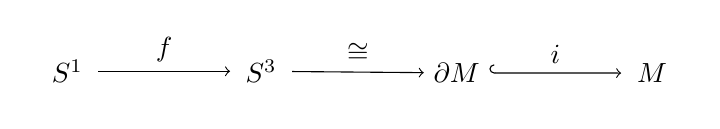
\begin{tikzpicture}
  \matrix (m) [matrix of math nodes, row sep=3.8em, column sep=4.8em, minimum width=2.2em]
  {
S^1 & S^3 & \partial M & M \\
};
  \path[->]
  (m-1-1) edge node [auto] {$f$} (m-1-2)
  (m-1-2) edge node [auto] {$\cong $} (m-1-3)
  ;
  \path[right hook->]
  (m-1-3) edge node [auto] {$i$} (m-1-4)
  ;
\end{tikzpicture}

Let us follow Hickerson (2013) \cite{Hick2013} to understand the number of approaches and models for ultracold neutrons \cite{Hick2013}.  

Consider the term
\[
\mathcal{L}_{\theta} = \frac{ \theta g^2}{ 8 \pi^2 } \text{tr}(F\wedge F) = \frac{ \theta g^2}{8 \pi^2} d\text{tr}( A \wedge dA + \frac{2}{3} A \wedge A \wedge A)
\]

We've seen how 
\begin{equation}
  \text{tr}(F_A \wedge F_A) \equiv \text{tr}(F\wedge F) = d\text{tr}(A \wedge dA + \frac{2}{3} A \wedge A \wedge A )
\end{equation}
is true, without regards to a \emph{metric} $g$ (or i.e. \emph{metric bundle} $g$ over $M$).  In pp. 5 Subsection 1.3 The $\theta$-term of Hickerson (2013) \cite{Hick2013}, the dual to $F$ was utilized.  Let's avoid utilizing ``electric-magnetic'' dual, or $g$, or Hodge dual terms in order to think purely ``topologically.''




\part{Preliminaries; (review of) Elementary concepts}


\section{Curvature}

Consider a principal-$G$ bundle with Lie group $G$, $P\xrightarrow{ \pi } M$.  Note that an associated bundle, a vector bundle, can be constructed from principal $G$-bundle $P$, through representation $\rho : G \to Gl(n;\mathbb{K})$ (cf. 10.9 Associated vector bundles of Taubes (2011) \cite{CTaubes2011}), in that 
\[
\begin{gathered}
\begin{tikzpicture}
  \matrix (m) [matrix of math nodes, row sep=3.8em, column sep=4.8em, minimum width=2.2em]
  {
P  \\
M  \\
};
  \path[->]
  (m-1-1) edge node [left] {$\pi$} (m-2-1)
  ;
\end{tikzpicture} \xrightarrow{ \rho : G \to \text{Gl}(n;\mathbb{K})} P \times_{\rho} \mathbb{K}^n \equiv P\times \mathbb{K}^n/(p,v)\sim (pg^{-1}, \rho(g)v) \quad \, \forall \, g \in G
\end{gathered}
\]
for $\mathbb{K} = \mathbb{R} \text{ or } \mathbb{C}$ and $\mathbb{K}^n$ being a vector space of dimension $n$ over field $\mathbb{K}$. 

Recall the exterior covariant derivative $D$ s.t.
\[
\begin{aligned}
  & D: \Omega^p(M;E) \to \Omega^{p+1}(M;E) \\ 
  & D(\theta \otimes s) = d\theta \otimes s + (-1)^p \theta \wedge \nabla s = d\theta \otimes s + \nabla s \wedge \theta
\end{aligned}
\]
with $E \xrightarrow{\pi} M$ being a vector bundle (from which one can construct the principal $G$ bundle, if so desired).  


\begin{proposition}
  For exterior covariant derivative $D: \Omega^p(M;E) \to \Omega^{p+1}(M;E)$, $\forall \, \eta \in \Omega^p(M;E)$, 
\[
D^2 \eta \equiv D\circ D \eta = F\wedge \eta
\]
where $F \in \Omega^p(M; \text{End}(E))$, and $F$ \emph{unique}
\end{proposition}

\begin{proof}
$\forall \, \eta \in \Omega^p(M;E)$, of the form $\eta = \theta \otimes s$, where $\theta \in \Omega^p(M)$, $s\in \Gamma(E)$, 
\[
\begin{gathered}
  D\eta = d\theta \otimes s + (-1)^p \theta \wedge \nabla s = d\theta \otimes s + (-1)^p \theta \wedge (ds + \omega^k_{ \; \; i } s^i e_k) = d\theta \otimes s + ds \wedge \theta + \omega^k_{ \; \; i} s^i \wedge \theta \otimes e_k = \\
  = (s^k d\theta + ds^k \wedge \theta + \omega^k_{ \; \; i } s^i \wedge \theta ) \otimes e_k 
\end{gathered}
\]
\[
\begin{gathered}
  D\circ D \eta \equiv DD\eta = (ds^k \wedge d\theta + (-1)ds^k \wedge d\theta + ds^i \wedge \omega^k_{ \; \; i} \wedge \theta + s^i d\omega^k_{ \; \; i } \wedge \theta + (-1) \omega^k_{ \; \; i} s^i \wedge d\theta ) \otimes e_k +\\
  + (-1)^{p+1}(s^k d\theta + ds^k \wedge \theta + \omega^k_{ \; \; i} s^i \wedge \theta ) \otimes \wedge \omega^l_{ \; \; k} e_l = \\
  = (ds^i \wedge \omega^l_{ \; \; i} \wedge \theta + s^i d\omega^l_{ \; \; i} \wedge \theta + (-1) \omega^l_{ \; \; i} s^i \wedge d\theta ) \otimes e_l + \\
  + (s^k \omega^l_{ \; \; k} \wedge d\theta + \omega^l_{ \; \; k } \wedge ds^k \wedge \theta + \omega^l_{ \; \; k} \wedge \omega^k_{ \; \; i } s^i \wedge \theta ) e_l = \\
  = (d\omega^l_{ \; \; i} + \omega^l_{ \; \; k } \wedge \omega^k_{ \; \; i} )s^i \wedge \theta e_l
\end{gathered}
\]
If you're following at home (i.e. independent study), one only needs to be careful with factors of $(-1)$ when ``commuting through'' the wedge product $\wedge$.  

I (still) find it a near miracle that terms cancel such that $F$ takes this form (with, simply a change of notation, $\omega \equiv A$):
\[
F = dA + A\wedge A \in \Omega^p(M;\text{End}E)
\]
By Lemma 11.1 of Sec. 11.2 the space of covariant derivatives of Taubes (2011) \cite{CTaubes2011}, this $F$ is \emph{unique}.  

Thus
\[
D^2 \eta = F \wedge \eta 
\]
for, notice that for, locally (in components)
\[
A = A^k_{ \; \; ij} dx^j \otimes (e_k \otimes e^i)
\]
\[
\begin{gathered}
  F = dA + A \wedge A = \frac{ \partial A^k_{ \; \; lj} }{  \partial x^i } dx^i \wedge dx^j \otimes (e_k \otimes e^l) + A^k_{  \; \; mi } A^m_{ \; \; lj } dx^i \wedge dx^j \otimes (e_k \otimes e^l) = \\
  = \left( \frac{ \partial A^k_{ \; \; lj} }{ \partial x^i} + A^k_{ \; \; mi} A^m_{ \; \; lj } \right) dx^i \wedge dx^j \otimes (e_k \otimes e^l )
\end{gathered}
\]
and so
\[
F\wedge \eta = \left( \frac{ \partial A^k_{ \; \; lj} }{ \partial x^i } + A^k_{ \; \; mi} A^m_{ \; \; lj } \right) dx^i \wedge dx^j \wedge \theta \otimes e_k s^l
\]
\end{proof}

\subsubsection{Alternative form of curvature $F$ in terms of commutators}
cf. Subsection 12.6 Curvature and commutators of Taubes (2011) \cite{CTaubes2011}.  

Consider $\forall \, U,V \in \mathfrak{X}(M)$, $X\in \Gamma(E)$,
\[
\nabla_U X = U^j \left( \frac{ \partial X}{ \partial x^j} + A^k_{ \; \; ij} X^i \right) = U^j \left( \frac{ \partial }{ \partial x^j } + A_j \right) X \in \Gamma(E)
\]
and so clearly 
\[
\nabla_U \in \Gamma(\text{End}(E))
\]
Also recall the commutator for vector fields, in component form (locally):
\[
[U,V] = \left( U^i \frac{ \partial }{ \partial x^i} V^j -  V^i \frac{ \partial }{ \partial x^i} U^j \right) \frac{ \partial }{ \partial x^j} \in \mathfrak{X}(M)
\]
and so 
\[
\nabla_{[U,V]} = \left( U^i \frac{ \partial }{ \partial x^i } V^j - V^i \frac{ \partial }{ \partial x^i } U^j \right) \left( \frac{ \partial }{ \partial x^j } + A_j \right)
\]
Consider that 
\[
\begin{gathered}
\nabla_U \nabla_V = \\
 = U^i \left[ \left( \frac{ \partial }{ \partial x^i } + A_i \right) V^j \left( \frac{ \partial }{ \partial x^j} + A_j \right) \right] = \\
  = U^i \left[  \frac{ \partial V^j}{ \partial x^i} \left( \frac{ \partial }{ \partial x^j} + A_j \right) + V^j \left( \frac{ \partial^2}{ \partial x^i \partial x^j } + \frac{ \partial A_j }{ \partial x^i } + A_j \frac{ \partial }{ \partial x^i } \right) + A_i V^j \frac{ \partial }{ \partial x^j} + A_i V^j A_j \right]
\end{gathered}
\]
Then by canceling out matching terms, 
\[
\begin{gathered}
  [ \nabla_U, \nabla_V ] - \nabla_{[U,V] } = U^i V^j \frac{ \partial A_j}{ \partial x^i} - V^i U^j \frac{ \partial A_j}{ \partial x^i} + U^i V^j A_i A_j - V^i U^j A_i A_j = \\
  = \left( \left( \frac{ \partial A_j }{ \partial x^i } - \frac{ \partial A_i}{ \partial x^j} \right) + [A_i, A_j] \right) U^i V^j = F(U,V)
\end{gathered}
\]
and so we have this form for the curvature $F(U,V) \in \Gamma(\text{End}(E))$, $\forall \, U,V \in \mathfrak{X}(M)$, 
\[
F(U,V) = \left( \left( \frac{ \partial A_j}{ \partial x^i } - \frac{ \partial A_i}{ \partial x^j } \right) + [A_i,A_j] \right)U^i V^j
\]
but I think that one should keep in mind that this is just one form that $F$ could take, if it is applied to $U,V$ beforehand.  

\subsubsection{deRham cohomology}

I'm going to now follow Section 12.2 Closed forms, exact forms, diffeomorphisms and De Rham cohomology of Taubes (2011) \cite{CTaubes2011}.  

Recall the definition of \emph{deRham cohomology}:
\begin{equation}
  H^p_{\text{deRham}}(M) := \text{ker}d/\text{im}d \qquad \, \left( = \lbrace \omega | d\omega = 0 \rbrace / \lbrace \theta | \theta = d\alpha \text{ for } \alpha \in \Omega^{p-1}(M) \rbrace \right)
\end{equation}

If $M,N$ smooth manifolds, smooth map $f: M \to N$, $\forall \, \alpha \in \Omega^{p-1}(N)$, then
\begin{equation}
  f^*(d\alpha ) =d(f^*\alpha) \text{ or } f^* d = df^*
\end{equation}
i.e.
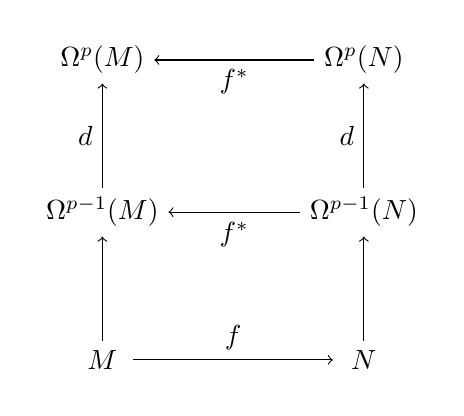
\begin{tikzpicture}
  \matrix (m) [matrix of math nodes, row sep=3.8em, column sep=4.8em, minimum width=2.2em]
  {
\Omega^p(M) & \Omega^p(N)  \\
\Omega^{p-1}(M) & \Omega^{p-1}(N)  \\
M & N   \\
};
  \path[->]
  (m-1-2) edge node [auto] {$f^*$} (m-1-1)
  (m-2-1) edge node [auto] {$d$} (m-1-1)
  (m-2-2) edge node [auto] {$d$} (m-1-2)
  edge node [auto] {$f^*$} (m-2-1)
  (m-3-1) edge node [auto] {$$} (m-2-1)
  edge node [auto] {$f$} (m-3-2)
  (m-3-2) edge node [auto] {$$} (m-2-2)
  ;
\end{tikzpicture}
\begin{proof}
Indeed, this can be shown, by considering local expressions: locally, $\alpha_I dy^I \in \Omega^{p-1}_y(N)$ where $I \equiv (i_1, i_2 \dots i_{p-1})$ s.t. $i_1 < i_2 < \dots < i_{p-1}$, and consider, with $f(x)=y$:
\[
\begin{gathered}
  \begin{aligned}
    & d\alpha = \frac{ \partial \alpha_I}{ \partial y^i} dy^i \wedge dy^I = \frac{ \partial \alpha_I}{\partial y^i} \epsilon^{iI }_J dy^J \text{ since there's only 1 way to permute $iI$ into $J=(j_1 \dots j_p)$ s.t. $j_1 < \dots < j_p$ } \\ 
    & f^*d\alpha = \frac{ \partial \alpha_I}{ \partial y^i} \epsilon^{iI}_J \frac{ \partial y^J}{ \partial x^k} dx^k \\ 
    & f^*\alpha = \alpha_I \frac{ \partial y^I}{ \partial x^J} dx^J = \frac{ \partial \alpha_I}{ \partial y^i} \frac{ \partial y^i }{ \partial x^j} \frac{ \partial y^I}{ \partial x^J} \epsilon^{jJ}_K dx^K
\end{aligned}
\end{gathered}
\]
Now
\[
\begin{gathered}
  df^* \alpha = \left( \frac{ \partial \alpha_I}{ \partial x^i} \frac{ \partial y^I}{ \partial x^j} + \alpha_I \frac{ \partial^2 y^I }{ \partial x^i \partial x^J} \right) dx^i \wedge dx^J = \left( \frac{ \partial \alpha_I}{ \partial x^i} \frac{ \partial y^I}{ \partial x^J} + \alpha_I \frac{ \partial^2 y^I}{ \partial x^i \partial x^J} \right) \epsilon^{iJ}_K dx^K = \\
  = \frac{ \partial \alpha_I}{ \partial y^i} \frac{ \partial y^i}{ \partial x^j} \frac{ \partial y^I}{ \partial x^J} \epsilon^{jJ}_K dx^K + \alpha_I  \frac{ \partial^2 y^J}{ \partial x^i  \partial x^J} \epsilon^{iJ}_K dx^K =  \frac{ \partial \alpha_I}{ \partial y^i} \frac{ \partial y^i}{ \partial x^j} \frac{ \partial y^I}{ \partial x^J} \epsilon^{jJ}_K dx^K + 0 = f^*d\alpha
\end{gathered}
\]
\end{proof}




Consider this homotopy: for smooth maps $\begin{aligned} & \quad \\
  & f_0: M \to N \\
  & f_1: M\to N \end{aligned}$, $\exists \,$ smooth map $\begin{aligned} & \quad \\
  & \psi : [0,1] \times M \to N \\
  & \psi(0, \cdot ) = f_0 \\
  & \psi(1,\cdot ) = f_1 \end{aligned}$

Let closed form $\omega \in \Omega^p(N)$; $d\omega= 0$.  Then $f_0^*\omega$, $f_1^* \omega$ closed form.  

Now consider $\mathbb{R} \times M$, and that 
\[
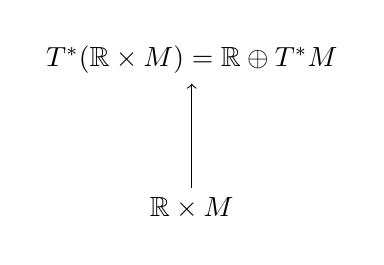
\begin{tikzpicture}
  \matrix (m) [matrix of math nodes, row sep=3.8em, column sep=4.8em, minimum width=2.2em]
  {
T^*(\mathbb{R} \times M) = \mathbb{R} \oplus T^*M \\
\mathbb{R} \times M \\
};
  \path[->]
  (m-2-1) edge node [auto] {$$} (m-1-1)
  ;
\end{tikzpicture} \text{ in that } 
\begin{tikzpicture}
  \matrix (m) [matrix of math nodes, row sep=3.8em, column sep=4.8em, minimum width=2.2em]
  {
\alpha = \alpha_0 dt + \alpha_M = \alpha_0 dt + (\alpha_M)_i dx^i \\
(t,x)  \\
};
  \path[->]
  (m-2-1) edge node [auto] {$$} (m-1-1)
  ;
\end{tikzpicture}
\]
in that $i$ runs through the indices for (some) local chart of $M$ \emph{only}, i.e. $i=1,2, \dots \text{dim}M=d$.  

Likewise, $\Omega^p(\mathbb{R} \times M) = \Omega^{p-1}(M) \oplus \Omega^p(M)$, in that 
\[
\begin{gathered}
 \forall \,  \alpha \in \Omega^p(\mathbb{R} \times M) \text{ then for $\mu = 0, 1, 2, \dots d$, $0$ standing in for $t\in \mathbb{R}$ of $\mathbb{R}\times M$, }\\ 
\alpha = \alpha_M dx^M = dt \wedge \alpha_I dx^I + \alpha_J dx^J \text{ where } \begin{aligned} & M = (\mu_1 \dots \mu_p) \quad & \mu_{\mu} = 0,1 \dots d \quad & \mu_1 < \dots < \mu_p \\
  & I = (i_1 \dots i_{p-1}) \quad & i_i = 1 \dots d \quad & i_1 < \dots < i_{p-1} \\
  & J = (j_1 \dots j_{p}) \quad & j_j = 1 \dots d \quad & j_1 < \dots < j_{p} 
\end{aligned} 
\end{gathered}
\]
and so, naming these components of $\alpha$ as 
\[
\begin{aligned}
  & \alpha^{p-1} \equiv \alpha_I dx^I \in \Omega^{p-1}(M) \\ 
  & \alpha^{p} \equiv \alpha_J dx^J \in \Omega^{p}(M) 
\end{aligned}
\]
Then $\forall \, \alpha \in \Omega^p(\mathbb{R} \times M)$, 
\begin{equation}\label{Eq:p-form}
\alpha = dt \wedge \alpha^{p-1} + \alpha^p
\end{equation}.  Taking $d$ on both sides to obtain $d\alpha \in \Omega^{p+1}(\mathbb{R} \times M)$, and $d\alpha$, being a $p+1$-form, taking the form of Eq. \ref{Eq:p-form}, then
\[
\begin{gathered}
  d\alpha = dt \wedge (d\alpha)^p + (d\alpha)^{p+1} = -dt \wedge d^{\perp} \alpha^{p-1} + \frac{ \partial \alpha^p_J}{ \partial t} dt \wedge dx^J + d^{\perp}\alpha^p
\end{gathered}
\]
where $d\alpha^p = \frac{ \partial \alpha^p_J}{ \partial x^{\mu }} dx^{\mu} \wedge dx^J = \frac{ \partial \alpha^p_J}{\partial t} dt \wedge dx^J + \frac{ \partial \alpha_J^p}{ \partial x^i} dx^i \wedge dx^J = \frac{ \partial \alpha_J^p }{ \partial t} dt \wedge dx^J + d^{\perp}\alpha^p$, and so $d^{\perp}$ signifies that this exterior derivative only ``acts'' on the (local) coordinates of $M$.  

Thus
\[
\begin{aligned}
  & (d\alpha)^p = -d^{\perp} \alpha^{p-1}  + \frac{ \partial \alpha^p }{ \partial t} \\ 
  &  (d\alpha)^{p+1} = d^{\perp}\alpha^p
\end{aligned}
\]

Suppose $\alpha = \psi^* \omega$; $\omega \in \Omega^p(N)$; $\psi : [0,1] \times M \to N$.  \\
If $\omega$ closed ($d\omega =0$), then $\psi^*\omega$ closed ($d\psi^* \omega = \psi^* d\omega =0$).  

So using the above facts shown for $\alpha = \psi^* \omega$,
\[
\begin{gathered}
\begin{aligned}
  & \alpha = dt \wedge \alpha^{p-1} + \alpha^p \xrightarrow{ \alpha = \psi^* \omega } \psi^* \omega = dt \wedge (\psi^* \omega)^{p-1} + (\psi^* \omega)^p \\ 
  &  d\psi^* \omega = \psi^* d\omega = 0 = dt \wedge (d\psi^* \omega)^p + (d\psi^* \omega)^{p+1}
\end{aligned} \\
\begin{aligned}
  &  (d\psi^* \omega)^{p+1} =0 = d^{\perp}(\psi^* \omega)^p \\ 
  & (d\psi^* \omega)^p = 0 = -d^{\perp}(\psi^* \omega)^{p-1} + \frac{ \partial ( \psi^* \omega)^p }{ \partial t} \xrightarrow{ \int_0^1 dt } \left. (\psi^* \omega)^p \right|_{t=1} - \left. (\psi^* \omega)^p \right|_{t=0} = d^{\perp} \int(\psi^* \omega)^{p-1} \text{ or } 
\end{aligned} \\
f_1^* \omega - f_0^* \omega = d^{\perp} \int (\psi^* \omega)^{p-1}
\end{gathered}
\]

So $f_1^* \omega$ differ from $f_0^* \omega$ by an exact form, $d^{\perp} \int(\psi^* \omega)^{p-1}$.  
\[
\Longrightarrow [f_1^* \omega] = [f_0^* \omega]
\]
Thus deRham cohomology classes are invariant under homotopy (homotopy invariant!).  

Consider 1-form connection on principal $G$-bundle $A=A(x) \in \Omega^1(M;\mathbf{g})$, $\forall \, x \in M$, $\mathfrak{g}$ Lie algebra of $G$ (Recall $\mathbf{g} = T_1G$).  \\
Consider 1-form connection over $[0,1] \times U$, open $U \subset M$, $A'=A'(t,x)$ in that
\[
A' = \mathbf{g}^{-1}d\mathbf{g} + t\mathbf{g}^{-1} A \mathbf{g} = A'(t,x)
\]
Note that $\mathbf{g} \in \mathfrak{g}$.  

$A'$ interpolates between a flat connection $A'(0,x) = \left. A' \right|_{t=0} = \mathbf{g}^{-1} d\mathbf{g}$, the connection 1-form for product principal bundle $P=M\times G$ and $A'(1,x) = \left. A'\right|_{t=1} = \mathbf{g}^{-1} d\mathbf{g} + \mathbf{g}^{-1} A \mathbf{g}$.  I think that this could be interpreted as turning off and turning on the gauge field, respectively.  

Now, doing the calculation out explicitly,
\[
\begin{gathered}
F_{A'} = (d+A')^2 = dA' + A'\wedge A' = d\mathbf{g}^{-1} \wedge d\mathbf{g} + dt \wedge \mathbf{g}^{-1} A \mathbf{g} + t(d\mathbf{g}^{-1} \wedge A \mathbf{g} + \mathbf{g}^{-1} dA \mathbf{g} + \mathbf{g}^{-1} A \wedge d\mathbf{g} + \\
 + t(\mathbf{g}^{-1} d\mathbf{g} \wedge \mathbf{g}^{-1} A \mathbf{g} + \mathbf{g}^{-1} A \mathbf{g} \wedge \mathbf{g}^{-1} d\mathbf{g} ) + t^2 \mathbf{g}^{-1} A \wedge A \mathbf{g}
\end{gathered}
\]
Using this identity:
\[
\begin{gathered}
  \mathbf{g}^{-1} \mathbf{g} = 1 \\ 
  \Longrightarrow d( \mathbf{g}^{-1} \mathbf{g} ) = d\mathbf{g}^{-1} \mathbf{g} + \mathbf{g}^{-1} d\mathbf{g} = 0 
\end{gathered}
\]
and ``commuting'' or ``moving through'' differential forms ``through the wedge product'', then
\[
F_{A'} = tdA + dt \wedge A + t^2 A \wedge A
\]

Now consider $\text{tr}(F_{A'} \wedge F_{A'} ) \in \Omega^4([0,1]\times U)$.  

$\text{tr}(F_{A'} \wedge F_{A'})$ is closed, since $\text{dim}M = 4$.  

Now recall that $\forall \, p$-form on $[0,1] \times U$, $\alpha \in \Omega^p([0,1]\times U)$, $\alpha = dt \wedge \alpha^{p-1} + \alpha^p$; with $\begin{aligned} & \quad \\ 
  & \alpha^{p-1} \in \Omega^{p-1}(U) \\
  & \alpha^p \in \Omega^p(U) \end{aligned}$

Thus, in our case currently, 
\[
\text{tr}(F_{A'} \wedge F_{A'}) = dt \wedge \alpha^3 + \alpha^4
\]
Calculating out $F_{A'} \wedge F_{A'}$ explicitly,
\[
\begin{gathered}
  F_{A'} \wedge F_{A'} = dt \wedge A \wedge tdA + t^3 A \wedge A \wedge dA + tdA \wedge dt \wedge A + t^2 dt \wedge A \wedge A \wedge A + \\
  + tdA \wedge A \wedge A + t^2 dt \wedge A \wedge A \wedge A =  \\
   = 2dt \wedge tA \wedge dA + 2 t^2 dt \wedge A \wedge A \wedge A + (t^3 + t) A\wedge A \wedge dA
\end{gathered}
\]
and so 
\[
\alpha^3 = 2\text{tr}(tA \wedge dA + t^2 A \wedge A \wedge A)
\]

Since $\text{tr}(F_{A'} \wedge F_{A'})$ closed, $0 = 0 - dt \wedge d\alpha^3 + d\alpha^4$, and ``applying'' $\frac{ \partial }{ \partial t}$ to this expression (i.e. this 4-form ``acts'' on $\frac{ \partial }{ \partial t}$, then 
\[
\begin{gathered}
  \frac{ \partial \alpha^4}{ \partial t} = d\alpha^3 \\ 
\xrightarrow{ \int dt } \int \frac{ \partial \alpha^4}{ \partial t} = \int d\alpha^3 = \text{tr}(F_{A'(1)} \wedge F_{A'(1)} ) - \text{tr}(F_{A'(0)} \wedge F_{A'(0) } ) = d\text{tr}(A\wedge dA + \frac{2}{3} A \wedge A \wedge A)
\end{gathered}
\]
Explicitly,
\[
\begin{gathered}
  d(\text{tr}(F_{A'} \wedge F_{A'}) ) = -dt \wedge d\alpha^3 + d\alpha^4 \\ 
  \xrightarrow{ \left( \frac{ \partial }{ \partial t} , \cdot, \cdot, \cdot \right) } \frac{ \partial ( \text{tr}(F_{A'} \wedge F_{A'} ) ) }{ \partial t} = - d\alpha^3 \xrightarrow{ \int_0^1 dt } \int_0^1 dt \frac{ \partial \text{tr}( F_{A'} \wedge F_{A'})}{ \partial t} = \int_0^1 dt ( -d\alpha^3)
\end{gathered}
\]
and so for $\text{tr}(F\wedge F) \in \Omega^4(M)$, $\text{tr}(A \wedge dA + \frac{2}{3} A \wedge A \wedge A) \in \Omega^3(M)$
\[
\Longrightarrow \text{tr}(F_A \wedge F_A) \equiv \text{tr}(F\wedge F) = d\text{tr}(A \wedge dA + \frac{2}{3} A \wedge A \wedge A )
\]
For oriented smooth $M$; $\text{dim}M=4$
\[
\int_M \text{tr}(F\wedge F)= \int_M d\text{tr}(A \wedge dA + \frac{2}{3} A \wedge A \wedge A ) = \int_{\partial M} \text{tr}(A \wedge dA + \frac{2}{3} A \wedge A \wedge A)
\]



Let us follow Hickerson (2013) \cite{Hick2013} to understand the number of approaches and models for ultracold neutrons \cite{Hick2013}.  

Consider the term
\[
\mathcal{L}_{\theta} = \frac{ \theta g^2}{ 8 \pi^2 } \text{tr}(F\wedge F) = \frac{ \theta g^2}{8 \pi^2} d\text{tr}( A \wedge dA + \frac{2}{3} A \wedge A \wedge A)
\]

We've seen how 
\begin{equation}
  \text{tr}(F_A \wedge F_A) \equiv \text{tr}(F\wedge F) = d\text{tr}(A \wedge dA + \frac{2}{3} A \wedge A \wedge A )
\end{equation}
is true, without regards to a \emph{metric} $g$ (or i.e. \emph{metric bundle} $g$ over $M$).  In pp. 5 Subsection 1.3 The $\theta$-term of Hickerson (2013) \cite{Hick2013}, the dual to $F$ was utilized.  Let's avoid utilizing ``electric-magnetic'' dual, or $g$, or Hodge dual terms in order to think purely ``topologically.''


\subsection{Geometry; Geometric setup; Manifold setup}

Following Eq. 1.28 on pp.5 of Subsection 1.3 The $\theta$-term of Hickerson (2013) \cite{Hick2013}, for a 3-cylinder $\partial M$, he has the following setup:
\[
\partial M = \mathbb{D}^3(t^+) \bigcup \mathbb{D}^3(t^-) \bigcup \mathbb{S}^2 \times \mathbb{R}
\]
Let's count dimensions.  
\[
\text{dim} \partial M  = \text{dim} \mathbb{D}^3(t^+) + \text{dim}\mathbb{S}^2 + 1 
\]
Now $\text{dim}\mathbb{S}^2 =2$.  So do we have more dimensions than allowed?  

Let's account for the various setups for a 4-dimensional topological gauge theory that involves knot polynomials (i.e. knot homologies).  It appears that Gaiotto and Witten (2011) \cite{GW2011} likes to include Riemann surfaces in $\partial M$, so there setup could be
\[
\partial M = \mathbb{C} \times \mathbb{R} (\text{or } \mathbb{C}\times S^1 (???) )
\]
where $\mathbb{C} \equiv $ Riemann surface (i.e. $f:\mathbb{C} \to \mathbb{C}$, $f$ holomorphic, i.e. $\begin{aligned} & \quad \\
  & \frac{ \partial f}{ \partial \overline{z}} = 0 \\
  & \frac{ \partial \overline{f}}{ \partial z } = 0 \end{aligned}$).  

\subsubsection{20160422 Things to do}

Clarify Manifold setup $\partial M \hookrightarrow M$; explore various manifold setups; pdf or equation of motion out of $\mathcal{L}$ and Euler-Lagrange equation and compare those equations to instanton equations of Gaiotto and Witten (2011) \cite{GW2011}; understand Virasoro algebra and conformal blocks for the quantum ``states'' that we can act upon; read more: Gaiotto and Witten (2011) \cite{GW2011}; Gukov (2007) \cite{Guko2007}, and of course classic Witten (1988) \cite{Witten:1988hf}


knot $K$ is an embedding $f: S^1 \to S^3$

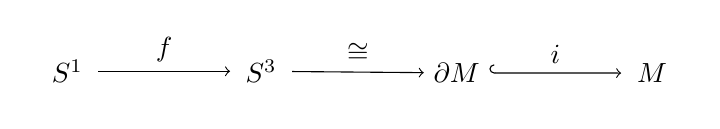
\begin{tikzpicture}
  \matrix (m) [matrix of math nodes, row sep=3.8em, column sep=4.8em, minimum width=2.2em]
  {
S^1 & S^3 & \partial M & M \\
};
  \path[->]
  (m-1-1) edge node [auto] {$f$} (m-1-2)
  (m-1-2) edge node [auto] {$\cong $} (m-1-3)
  ;
  \path[right hook->]
  (m-1-3) edge node [auto] {$i$} (m-1-4)
  ;
\end{tikzpicture}


%\[
%\begin{fmffile}{simple}
%    \begin{fmfgraph}(150,60)
       % Note that the size is given in normal parentheses
       % instead of curly brackets.
       % Define external vertices from bottom to top
%        \fmfleft{i1,i2}
%        \fmfright{o1,o2}
%        \fmf{fermion}{i1,v1,o1}
%        \fmf{fermion}{i2,v2,o2}
%        \fmf{photon}{v1,v2}
%   \end{fmfgraph}
%\end{fmffile}
%\]

% \begin{fmffile}{simple}
%  \begin{fmfgraph}(150,60)
    
    % Define external vertices from bottom to top


%    \fmfleft{i1}
%    \fmfright{o1,o2}

%    \fmf{fermion}{i1,v1}
%    \fmf{gluon}{v1,v2}
%    \fmf{gluon}{v2,v3}
%    \fmf{gluon}{v3,v1}
%    \fmf{fermion}{v2,o1}
%    \fmf{fermion}{v3,o2}

%    \fmfdot{v1}
%    \fmfdot{v2}
%    \fmfdot{v3}

%  \end{fmfgraph}
%\end{fmffile}


\subsection{Reviewing Witten's Quantum Field Theory and the Jones Polynomial}

Let's review Witten's seminal paper (of which he won a Fields medal for, and is, as of 20160503, the only physicist to have won the Fields medal) (cf. Witten (1988) \cite{Witten:1988hf}).  

Note that this is \emph{not} a perturbative theory, i.e. no \emph{perturbations} were used.  This is a non-perturbative theory yielding \emph{exact} solutions, exact topological solutions, i.e. with deal relation to topology.  \textbf{Conformal Field Theory} was employed in the quantization.  Thus, tools from conformal field theory are needed and maybe very unfamiliar to someone that was raised in the usual quantum field theory class with Feynman diagrams.  Thus, a generous amount of time will be taken to understand \emph{conformal field theory}.  

Witten uses the following setup:\cite{Witten:1988hf}

Given an oriented 3-manifold $M$, $\text{dim}M=3$, and \\
compact simple gauge group $G$ (simple being no nontrivial ideals),

then the following Lagrangian was considered
\[
\mathcal{L} = \frac{k}{4\pi} \int_M \text{tr}(A \wedge dA + \frac{2}{3} A \wedge A \wedge A ) \equiv \frac{k}{4\pi } \int_M \text{tr}(AdA + \frac{2}{3}A^3)
\]

Witten then references that the \emph{quantization law} was first discussed in Deser, Jackiw, Templeton (1982) \cite{DJT1982}.

Because group $\widehat{G}$ of cont. maps $M \to G$ not connected, $\widehat{G} = \mathcal{C}^1(M;G)$  \\
\phantom{\qquad} then at least $\pi_3(G) \simeq \mathbb{Z}$\, $\forall \, $ compact simple (again, meaning no nontrivial ideals) group $G$.  

$\mathcal{L} = \frac{k}{4\pi } \int_M \text{tr}(AdA + \frac{2}{3} A^3)$ invariant under component of gauge group that contains identity, $(T_eG \equiv T_1G \equiv \mathfrak{g}$), \\

$\mathcal{L}$ is not invariant under gauge transformations associated with nonzero elements of $\pi_3(G)$ (nonzero ``winding number'') (???)
\[
\mathcal{L} \mapsto \mathcal{L} + \text{const.}m
\]
As in Dirac's famous work in magnetic monopoles, QFT requires  single-valuedness of $\exp{(i\mathcal{L})} \mapsto \exp{(i(\mathcal{L} + 2\pi k )) }$ (quantization condition on $k$ in $\mathcal{L}$)

We have $G=SU(N)$, and trace over representations
\[
\text{tr}(A^3) \equiv \text{tr}(A\wedge A \wedge A) = A^a_{\; \; bi } A^{b \; \; cj} A^c_{ \; \; ak} dx^i \wedge dx^j \wedge dx^k
\]
Witten considered the entire time that $A$ is in the \emph{fundamental representation} of \emph{$N$ dimensions}.

Recall that the fundamental representation is a homomorphism $\begin{aligned} & \quad \\
  & \rho : G \to G \\ & \rho(g)=g \end{aligned}$
and it happens to be in this case, with $G=SU(N)$, that $G$ is also an endomorphism on vector space $V$, $G=\text{End}V$ with $\text{dim}V=N$, where $V$ is called by some the ``representation space.''  For the $N=2$ case, then $\rho(g)=g$ are the usual $2\times 2$ special unitary matrices, $\forall \, g \in SU(2)$, which act on the 2-dim. vector space $V_2$ of basis spin-up and spin-down vectors (``doublets'').  It maybe interesting to extend this to other ``spin'' representations i.e. $\rho:G \to \text{End}(V)$ with $\text{dim}V > N$, or clarify what the adjoint representation means to this case.

Nevertheless, keeping in mind that the fundamental representation is only considered, \\
$k$ is very closely related to the central charge in the highest weight representations of affine Lie algebras (promised later in the paper)

We wish to pick a suitable class of gauge invariant observables that \emph{also} are ``topologically invariant'' or ``generally covariant'' or ``manifestly covariant'' (they mean the same thing).  \\
$\Longrightarrow $ Wilson line $W$.  

Let $R$ be irrep (irreducible representation) of $G$.  Let $K \equiv $ knot, i.e. embedding of $S^1$ in $M^3$; knot $K$ can be a circle $S^1$, in this case it's called the ``unknot''.
\[
W_R(K) := \text{tr}_R P\exp{ \int_K A}
\]
link $L := \coprod_{i=1}^r K_i $; $K_i$ oriented and non-intersecting knot.

Calculate Feynman path integral $\int \mathcal{D}\mathcal{A} \exp{ (i\mathcal{L})} \coprod_{i=1}^r W_{R_i}(K_i) = \langle \coprod_{i=1}^r W_{R_i}(K_i) \rangle$, \\
  with $\int D\mathcal{A} \equiv $ Feynman's integral over all gauge orbits i.e. over $\mathcal{A}/\mathcal{G}$ i.e. equivalence classes of connections modulo gauge transformations.

So now we get a partition function:
  \[
\langle \prod_{i=1}^r W_{R_i}(K_i) \rangle \equiv Z(M; K_i , R_i) \equiv Z(M;L)
\]

In Witten's second point, (2), for his intuition that this is the correct form, is this: considering reverse orientation of $1$ $K_i$, simultaneously exchange representation $R_i$ with complex conjugate $\overline{R}_i$, $Z(M;K_i,R_i)$ invariant.  \\
``charge conjugation'' reverse orientation $\forall \l K_i $ of $L \Longrightarrow $ involution of $\mathfrak{g}$, exchange all representation $R_i$ with their conjugates.

Now
\[
Z = \int \mathcal{D}\mathcal{A} \exp{ \left( \frac{ik}{4\pi } \int_{M^3} \text{tr}(AdA + \frac{2}{3} A^3) \right) }
\]
wildly oscillates (due to $k$).

Stationary pts. of Chern-Simons action are (``flat connections''), $F\in \Omega^2(M;\mathfrak{g})$, $F\equiv F_A(x) = 0$.

From Witten, referencing ref. [18], Ray-Singer analytic torsion of flat connection $A^{(\alpha)}$ is topological invariant, and so is $\mu(A^{(\alpha)})$ in $Z=\sum_{\alpha} \mu(A^{(\alpha)}$ (for large $k$).

(to be continued)
  

  


\subsubsection{Framing}

(to be continued)


Witten introduces in Eq. (4.21) \cite{Witten:1988hf} the parameter $q$
\[
q = \exp{ \left( \frac{2\pi i }{ N + k } \right) }
\]
(still in consideration of $S^3$).

For $G=SU(2)$, integrable representations of level $k$ are those of spin $n/2$, $n=0 \dots k$
\[
S_{mn} = \sqrt{ \frac{2}{k+2} } \sin{\left( \frac{ (m+1)(n+1)\pi }{ k+2} \right) }
\]
For spin $0$, $n=0$, $S_{m0} = \sqrt{ \frac{2}{k+2} } \sin{ \left( \frac{ (m+1) \pi  }{ k+2} \right) }$  \\
For spin $1/2$, $n=1$, $S_{m1} = \sqrt{ \frac{2}{k+2} } \sin{ \left( \frac{ (m+1) 2\pi  }{ k+2} \right) }$  \\
For spin $1$, $n=2$, $S_{m2} = \sqrt{ \frac{2}{k+2} } \sin{ \left( \frac{ (m+1) 3\pi  }{ k+2} \right) }$

From pp. 362, ``Some Examples'' subsection of Sec. 2 of Witten \cite{Witten:1988hf}, $Z(S^2 \times S^1) =1$ \, $\forall \, G, \, \forall k$.
\[
Z(S^3)=\sqrt{ \frac{2}{k+2} } \sin{ \left( \frac{ \pi}{k+2} \right)} = S_{00}; \, m,n=0
\]


\section{Calculations (so far)}

Consider the action
\begin{equation}
  %  S = \exp{ (i \mathcal{L}_{KE} + i \mathcal{L}_{\theta} ) } = \exp{ (i\mathcal{L}_{KE})} \exp{ (i\mathcal{L}_{\theta} ) }
  S = \exp{ (i L_{KE} + i L_{\theta} ) } = \exp{ (i L_{KE})} \exp{ (i L_{\theta} ) }
\end{equation}
Suppose
\[
L_{KE} = \int_{M^4} \text{tr}(F\wedge * F)
\]
where $M^4$ is a 4-manifold, $\text{dim}M^4=4$ and $M^4$ is a smooth, Lorentzian manifold.  

For the $L_{\theta}$ term,
\[
\begin{gathered}
  L_{\theta} = \int_{M^4} \frac{ \theta g^2}{8\pi^2} \text{tr}(F\wedge F) = \int_{M^4} \frac{ \theta g^2}{8 \pi^2} d\text{tr}(A\wedge dA + \frac{2}{3} A \wedge A \wedge A ) = \int_{M^3 = \partial M^4} \frac{ \theta g^2}{8 \pi^2} \text{tr}(A\wedge dA + \frac{2}{3} A\wedge A \wedge A )
  \end{gathered}
\]

How do we deal with the ``foliation'' of $M^4$ to a 3-manifold for the boundary of $M^4$, $M^3 = \partial M^4$?  Possibly, one could ``choose a gauge'' s.t. $A_0 =0$.  So if we want our knots to propagate in time $t=x^0$, then $M^3 = \partial M^4$ is the ``physical'' space of spacetime, our usual 3-dimensions of space.  However, it appears that Witten \cite{Witten:1988hf} treats a $2+1$-dim. Yang-Mills theory, and so $M^3$ 3-manifold has time mixed up in it.  Also, are we considering Wilson loops being trajectories of fermions over time?  Or Wilson loops through 3-dimension physical space and see how the knots evolve over time?  I'm still not clear about which way to go.

If we proceed with
\begin{equation}
\begin{gathered}
  L_{\theta} = \int_{M^3 = \partial M^4} \frac{ \theta g^2}{8 \pi^2} \text{tr}(A\wedge dA + \frac{2}{3} A\wedge A \wedge A ) \\ 
  S = \exp{ i L_{\theta}}
  \end{gathered}
\end{equation}
In light of the quantization condition, this imposes conditions on $L_{\theta}$:
\[
L_{\theta} \mapsto L_{\theta} + \text{const.} \cdot m
\]
then we can identify the level $k$ in such a way:
\[
\frac{k}{4\pi} = \frac{\theta g^2}{ 8\pi^2} \Longrightarrow k = \frac{\theta g^2}{2\pi}
\]
We can calculate the expectation values of Wilson lines of various torus knots (which, keep in mind, are denoted as partition functions, $Z$) (EY: 20160508 I'll have to check the normalization over the partition function of the unknot i.e. the expectation value of the Wilson line of the unknot, $Z(S^1)$).  I myself, using the Khovanov homology package  \verb|knotkh|, or one can use SnapPy, and I've implemented with SnapPy as well, so you can use SnapPy in equal manner for only the Jones polynomial, have calculated the Jones polynomial, with Khovanov homology, for torus knots of less than 14 crossings (I can do more, but my MacBook Air ``crapped'' out), 9 of them:
\[
\begin{aligned}
  & T(2,1) \\ 
  & T(2,3) \\ 
  & T(2,5) \\ 
  & T(2,7) \\ 
  & T(2,9) \\ 
  & T(2,11) \\ 
  & T(2,13) \\ 
  & T(3,4) \\ 
  & T(3,5) 
  \end{aligned}
\]
Let me show examples for $T(2,1)$, $T(2,3)$, % $T(2,5)$.

The respective Jones polynomial for $T(2,1)$, $T(2,3)$, $T(2,5)$, which, on the quantum field theory side, Chern-Simons on 3-manifold for $SU(N)$ gauge group, in the fundamental representation, is the expectation value of the Wilson line or partition function, $Z(T(2,1))$, $Z(T(2,3))$, $Z(T(2,5))$,
\[
\begin{aligned}
  & Z(T(2,1)) = \frac{q^{2} + 1}{q}    \\
  & Z(T(2,3)) = q^{9}  + q^{7}  + q^{7}  + q^{5}  + q^{3} + q \\  
  & Z(T(2,5)) = q^{15}  + q^{13}  + q^{13}  + q^{11}  + q^{11}  + q^{9}  + q^{9}  + q^{7}  + q^{5} + q^{3}  
\end{aligned}
\]
I should remark that these Jones polynomials are simply the special case of when $t=1$ in the Khovanov homology:
\[
\begin{aligned}
  & Z(T(2,1);q,t) = \frac{q^{2} + 1}{q}    \\
  & Z(T(2,3);q,t) = q^{9} t^{3} + q^{7} t^{3} + q^{7} t^{2} + q^{5} t^{2} + q^{3} + q \\  
  & Z(T(2,5);q,t) = q^{15} t^{5} + q^{13} t^{5} + q^{13} t^{4} + q^{11} t^{4} + q^{11} t^{3} + q^{9} t^{3} + q^{9} t^{2} + q^{7} t^{2} + q^{5} + q^{3}  
\end{aligned}
\]
For level $k = \frac{\theta g^2}{2\pi}$, and from Witten's introduction \cite{Witten:1988hf} of $q$, $q = \exp{ \left( \frac{2\pi i}{ N+k} \right)}$, then for $SU(2)$ (i.e. $N=2$),

for $Z(T(2,1);q,t)$,
\[
Z(T(2,1);q,t) = {\left(e^{\left(\frac{8 i \, \pi}{\frac{g^{2} \theta}{\pi} + 4}\right)} + 1\right)} e^{\left(-\frac{4 i \, \pi}{\frac{g^{2} \theta}{\pi} + 4}\right)}
\]
and for the real part:
\[
\begin{gathered}
\Re Z(T(2,1);q,t) =   \cos\left(\frac{4 \, \pi}{\frac{g^{2} \theta}{\pi} + 4}\right) + \cos\left(-\frac{4 \, \pi}{\frac{g^{2} \theta}{\pi} + 4}\right)
  \end{gathered}
\]
and for the imaginary part:
\[
\begin{gathered}
  \Im Z(T(2,1);q,t) = \sin\left(\frac{4 \, \pi}{\frac{g^{2} \theta}{\pi} + 4}\right) + \sin\left(-\frac{4 \, \pi}{\frac{g^{2} \theta}{\pi} + 4}\right)
  \end{gathered}
\]

For $Z(T(2,3);q,t)$,
\[
Z(T(2,3);q,t) = t^{3} e^{\left(\frac{36 i \, \pi}{\frac{g^{2} \theta}{\pi} + 4}\right)} + t^{3} e^{\left(\frac{28 i \, \pi}{\frac{g^{2} \theta}{\pi} + 4}\right)} + t^{2} e^{\left(\frac{28 i \, \pi}{\frac{g^{2} \theta}{\pi} + 4}\right)} + t^{2} e^{\left(\frac{20 i \, \pi}{\frac{g^{2} \theta}{\pi} + 4}\right)} + e^{\left(\frac{12 i \, \pi}{\frac{g^{2} \theta}{\pi} + 4}\right)} + e^{\left(\frac{4 i \, \pi}{\frac{g^{2} \theta}{\pi} + 4}\right)}
\]
and for the real part:




\newpage


\[
\begin{gathered}
  \Re Z(T(2,3);q,t) = \\
\end{gathered}
\]
  \begin{dmath}
  -3 \, \cos\left(\frac{36 \, \pi}{\frac{g^{2} \theta}{\pi} + 4}\right) \Im \left( t \right)^{2} \Re \left( t \right) - 3 \, \cos\left(\frac{28 \, \pi}{\frac{g^{2} \theta}{\pi} + 4}\right) \Im \left( t \right)^{2} \Re \left( t \right) + \cos\left(\frac{36 \, \pi}{\frac{g^{2} \theta}{\pi} + 4}\right) \Re \left( t \right)^{3} + \cos\left(\frac{28 \, \pi}{\frac{g^{2} \theta}{\pi} + 4}\right) \Re \left( t \right)^{3} + \Im \left( t \right)^{3} \sin\left(\frac{36 \, \pi}{\frac{g^{2} \theta}{\pi} + 4}\right) - 3 \, \Im \left( t \right) \Re \left( t \right)^{2} \sin\left(\frac{36 \, \pi}{\frac{g^{2} \theta}{\pi} + 4}\right) + \Im \left( t \right)^{3} \sin\left(\frac{28 \, \pi}{\frac{g^{2} \theta}{\pi} + 4}\right) - 3 \, \Im \left( t \right) \Re \left( t \right)^{2} \sin\left(\frac{28 \, \pi}{\frac{g^{2} \theta}{\pi} + 4}\right) - \cos\left(\frac{28 \, \pi}{\frac{g^{2} \theta}{\pi} + 4}\right) \Im \left( t \right)^{2} - \cos\left(\frac{20 \, \pi}{\frac{g^{2} \theta}{\pi} + 4}\right) \Im \left( t \right)^{2} + \cos\left(\frac{28 \, \pi}{\frac{g^{2} \theta}{\pi} + 4}\right) \Re \left( t \right)^{2} + \cos\left(\frac{20 \, \pi}{\frac{g^{2} \theta}{\pi} + 4}\right) \Re \left( t \right)^{2} - 2 \, \Im \left( t \right) \Re \left( t \right) \sin\left(\frac{28 \, \pi}{\frac{g^{2} \theta}{\pi} + 4}\right) - 2 \, \Im \left( t \right) \Re \left( t \right) \sin\left(\frac{20 \, \pi}{\frac{g^{2} \theta}{\pi} + 4}\right) + \cos\left(\frac{12 \, \pi}{\frac{g^{2} \theta}{\pi} + 4}\right) + \cos\left(\frac{4 \, \pi}{\frac{g^{2} \theta}{\pi} + 4}\right)
\end{dmath}

\quad \\ 
  

\quad \\
and for the imaginary part: 

\quad \\ 

\[
\begin{gathered}
  \Im Z(T(2,3);q,t) = \\
\end{gathered}
\]
  \begin{dmath}  -\cos\left(\frac{36 \, \pi}{\frac{g^{2} \theta}{\pi} + 4}\right) \Im \left( t \right)^{3} - \cos\left(\frac{28 \, \pi}{\frac{g^{2} \theta}{\pi} + 4}\right) \Im \left( t \right)^{3} + 3 \, \cos\left(\frac{36 \, \pi}{\frac{g^{2} \theta}{\pi} + 4}\right) \Im \left( t \right) \Re \left( t \right)^{2} + 3 \, \cos\left(\frac{28 \, \pi}{\frac{g^{2} \theta}{\pi} + 4}\right) \Im \left( t \right) \Re \left( t \right)^{2} - 3 \, \Im \left( t \right)^{2} \Re \left( t \right) \sin\left(\frac{36 \, \pi}{\frac{g^{2} \theta}{\pi} + 4}\right) + \Re \left( t \right)^{3} \sin\left(\frac{36 \, \pi}{\frac{g^{2} \theta}{\pi} + 4}\right) - 3 \, \Im \left( t \right)^{2} \Re \left( t \right) \sin\left(\frac{28 \, \pi}{\frac{g^{2} \theta}{\pi} + 4}\right) + \Re \left( t \right)^{3} \sin\left(\frac{28 \, \pi}{\frac{g^{2} \theta}{\pi} + 4}\right) + 2 \, \cos\left(\frac{28 \, \pi}{\frac{g^{2} \theta}{\pi} + 4}\right) \Im \left( t \right) \Re \left( t \right) + 2 \, \cos\left(\frac{20 \, \pi}{\frac{g^{2} \theta}{\pi} + 4}\right) \Im \left( t \right) \Re \left( t \right) - \Im \left( t \right)^{2} \sin\left(\frac{28 \, \pi}{\frac{g^{2} \theta}{\pi} + 4}\right) + \Re \left( t \right)^{2} \sin\left(\frac{28 \, \pi}{\frac{g^{2} \theta}{\pi} + 4}\right) - \Im \left( t \right)^{2} \sin\left(\frac{20 \, \pi}{\frac{g^{2} \theta}{\pi} + 4}\right) + \Re \left( t \right)^{2} \sin\left(\frac{20 \, \pi}{\frac{g^{2} \theta}{\pi} + 4}\right) + \sin\left(\frac{12 \, \pi}{\frac{g^{2} \theta}{\pi} + 4}\right) + \sin\left(\frac{4 \, \pi}{\frac{g^{2} \theta}{\pi} + 4}\right)
  \end{dmath}

  (Breaking up multiple line latex output from Sage Math is a pain and for some reason, the latex environment dmath isn't working here; at this point, and in general, I would go to the \url{https://github.com/ernestyalumni/qSApoly/blob/master/JonesPoly_and_KH/JonesPolyetKH_sage.ipynb}

  %{\verb|JonesPolyetKH_sage.ipynb|}

  jupyter notebook and see that it's all there. 
  


\newpage



  If one substitutes in $t=1$ for $Z(T(2,3);q,t)$, then
  \[
\begin{gathered}
  Z(T(2,3);q,t=1) = \\
e^{\left(\frac{36 i \, \pi}{\frac{g^{2} \theta}{\pi} + 4}\right)} + 2 \, e^{\left(\frac{28 i \, \pi}{\frac{g^{2} \theta}{\pi} + 4}\right)} + e^{\left(\frac{20 i \, \pi}{\frac{g^{2} \theta}{\pi} + 4}\right)} + e^{\left(\frac{12 i \, \pi}{\frac{g^{2} \theta}{\pi} + 4}\right)} + e^{\left(\frac{4 i \, \pi}{\frac{g^{2} \theta}{\pi} + 4}\right)}
\end{gathered}
\]
and for the real part,
\[
\begin{gathered}
  \cos\left(\frac{36 \, \pi}{\frac{g^{2} \theta}{\pi} + 4}\right) + 2 \, \cos\left(\frac{28 \, \pi}{\frac{g^{2} \theta}{\pi} + 4}\right) + \cos\left(\frac{20 \, \pi}{\frac{g^{2} \theta}{\pi} + 4}\right) + \cos\left(\frac{12 \, \pi}{\frac{g^{2} \theta}{\pi} + 4}\right) + \cos\left(\frac{4 \, \pi}{\frac{g^{2} \theta}{\pi} + 4}\right)
  \end{gathered}
\]
and for the imaginary part,
\[
\begin{gathered}
\sin\left(\frac{36 \, \pi}{\frac{g^{2} \theta}{\pi} + 4}\right) + 2 \, \sin\left(\frac{28 \, \pi}{\frac{g^{2} \theta}{\pi} + 4}\right) + \sin\left(\frac{20 \, \pi}{\frac{g^{2} \theta}{\pi} + 4}\right) + \sin\left(\frac{12 \, \pi}{\frac{g^{2} \theta}{\pi} + 4}\right) + \sin\left(\frac{4 \, \pi}{\frac{g^{2} \theta}{\pi} + 4}\right)
  \end{gathered}
\]
Again, all the calculations, and further full expressions are in the jupyter notebook page (which requires Sage Math), with all the symbolic computations, called \url{https://github.com/ernestyalumni/qSApoly/blob/master/JonesPoly_and_KH/JonesPolyetKH_sage.ipynb}

%{\verb|JonesPoly_and_KH.ipynb|}.  





\section{Standard Model}

From \emph{Wikipedia}, on ``Standard Model (mathematical formulation)'', (cf. \url{https://en.wikipedia.org/wiki/Standard_Model_(mathematical_formulation)}), they have a nice and neat chart of the field content of the standard model (SM) and I'll reproduce the gauge fields table:

%\begin{table}
%\centering
\begin{tabular}{l c c c r }
\multicolumn{5}{c}{Field content of the standard model (SM)} \\
\multicolumn{5}{c}{Spin 1 - gauge fields } \\
Symbol & Associated charge & Group & Coupling & Representation \\ 
$B$ & Weak hypercharge & $U(1)_Y$ & $g'$ & $( \mathbf{1}, \mathbf{1}, 0)$ \\
$W$ & Weak isospin & $SU(2)_L$ & $g_w$   & $(\mathbf{1}, \mathbf{3} , 0 )$ \\ 
$G$ & Color & $SU(3)_C$ & $g_s$ & $(\mathbf{8}, \mathbf{1}, 0)$  \\
\end{tabular}
%\end{table}

\subsubsection{Representation for SM}

As a warmup, consider the group $GL(N,\mathbb{C})$:
\[
GL(N;\mathbb{C}) = \lbrace X | X \in \text{Mat}_{\mathbb{C}}(N,N), \text{det}X \neq 0 \rbrace
\]
where $\text{Mat}_{\mathbb{C}}(N,N)$ denotes the space (not group) of all $N\times N$ matrices with complex numbers in (all of) its entries.

Clearly, 
\[
\begin{aligned}
  & \text{dim}_{\mathbb{C}}GL(N;\mathbb{C}) = N^2 \\ 
  & \text{dim}_{\mathbb{R}}GL(N;\mathbb{C}) = 2*N^2 = 2N^2 \quad \, (\text{for the 2 real numbers for \emph{each} complex entry})
\end{aligned}
\]
where I denote whether we're talking about \emph{complex} dimensions (i.e. in using complex numbers) or dimension with real numbers; hence the subscript under $\text{dim}$.  

Consider 
\[
U(N) = \lbrace U \in GL(N,\mathbb{C} | UU^{\dag} = 1\rbrace
\]
Now
\begin{proposition}
  \[
\begin{aligned}
& \text{dim}_{\mathbb{R}}U(N) = N^2
& \text{dim}_{\mathbb{R}}SU(N) = N^2 -1
\end{aligned}
\]
\end{proposition}
\begin{proof}
A great way to calculate this is found in \url{http://www.phys.nthu.edu.tw/~class/Group_theory/Chap%207.pdf}, pp. 112, Chapter 7 Classical Lie Groups.  

Each row of $\forall \, U \in U(N)$ has unit norm (analogous to $O(N)$), and different rows are ``orthogonal'', with respect to some inner product.  

First row determined by $N$ complex numbers (parameters), or $2N$ real numbers.  \\
\phantom{First} subtract 1 for unit norm condition.  $2N-1$.  

2nd row determined by $N-1$ complex numbers; orthgonality determined by one of the complex numbers (parameters).  So $2N-2$ real numbers. \\
\phantom{First} subtract 1 for unit norm condition: $2N-3$.  

Thus,
\[
\sum_{j=1}^N 2N - (2j - 1) = 2N^2 - 2\left( \frac{N(N+1)}{2} \right)  + N = N^2
\]
For $SU(N)$, $\text{det}SU(N) =1$.  This fixes the overall phase of $\text{det}X$, $X\in SU(N)$ (since $\text{det}(UU^{\dag}) = \text{det}U \text{det}U^{\dag} = 1$ and so $\text{det}U$ has norm $1$, i.e. $|\text{det}U|=1$, $\forall \, U \in U(N)$, already).  So that costs another \emph{real} number (parameter).  So for $SU(N)$, $N^2-1$ \emph{real} number parameters are independent.  

\end{proof}

Recall that an automorphism is an isomorphism from a mathematical object to itself.  Denote $\text{Aut}(V)$ to be the space of all possible automorphisms on mathematical object $V$ (prominent example is vector space $V$).  


From L\"{o}h's notes on representation theory of Lie algebra (cf. Clara L\"{o}h ``Representation theory of Lie algebra.''  \url{http://deferentialgeometry.org/papers/Loeh%20-%20Representation%20Theory%20of%20Lie%20Algebras.pdf}), 

if (given) $\phi : G \to \text{Aut}(V)$ is a representation of $G$, then $T_1 \phi : \mathfrak{g} \to \text{End}(V)$ is a representation of the Lie algebra, i.e. making
\[
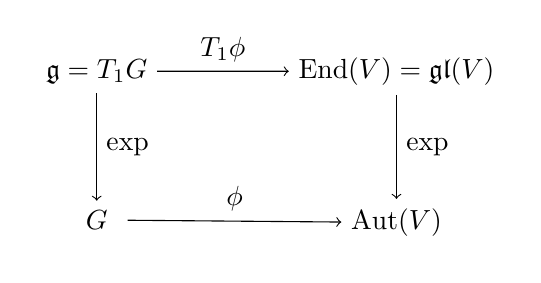
\begin{tikzpicture}
  \matrix (m) [matrix of math nodes, row sep=3.8em, column sep=4.8em, minimum width=2.2em]
  {
\mathfrak{g} = T_1 G  & \text{End}(V) = \mathfrak{gl}(V) \\ 
G & \text{Aut}(V) \\ 
};
  \path[->]
  (m-1-1) edge node [auto] {$T_1\phi$} (m-1-2)
  edge node [auto] {$\exp $ } (m-2-1)
  (m-1-2) edge node [auto] {$\exp $} (m-2-2)
  (m-2-1) edge node [auto] {$\phi$ } (m-2-2)
;
\end{tikzpicture}
\]
Since $SU(N)$ is simply connected (recall, $\text{det}A =1 \, \forall \, A \in SU(N)$, by definition, and so $\text{det}:SU(N) \to \mathbb{C}$, being a continuous function, and with the preimage of $\lbrace 1 \rbrace$, $\text{det}^{-1}(\lbrace 1 \rbrace)$, being the entire $SU(N)$, and $\lbrace 1 \rbrace$, clearly a closed set, then $SU(N)$ simply connected).  Note that $U(N)$ is not simply connected.  Note that this has a good chart of simply connected vs. not simply connected: \href{http://www.google.com/url?q=http://www.springer.com/cda/content/document/cda_downloaddocument/9780387401225-c1.pdf%3FSGWID%3D0-0-45-164608-p7110377&sa=U&ved=0ahUKEwix0ZbriMLMAhUD62MKHbcJCvcQFggUMAA&usg=AFQjCNEK0TttSALM_ecQrQfNRQeoC2WwSw}{1 Matrix Lie Groups - Springer}, we can go the other way, in that 

given representation of Lie algebra $\mathfrak{g}$, say $\rho : \mathfrak{g} \to Gl(V)$, $\exists \, \exp{(\rho)}:G \to \text{Aut}(V)$ group representation.  

Ciaran Hughes makes the poignant remark/observation in distinguishing the \emph{representation space} (cf. \href{http://www.damtp.cam.ac.uk/user/ch558/pdf/Representations.pdf}{A brief discussion on representations}.  While 
\[
\begin{aligned}
  \text{dim}(SU(N)) = N^2 - 1 &   \text{dim}(\mathfrak{su}(N)) = N^2 - 1 \\
  \text{dim}(SU(2)) = 3       &   \text{dim}(\mathfrak{su}(2)) = 3 \\
  \text{dim}(SU(3)) = 8       &   \text{dim}(\mathfrak{su}(3)) = 8 
\end{aligned}
\]
so the dimensions of $SU(N)$ and corresponding $\mathfrak{su}(N)$ \emph{look} equal, but they were arrived at from entirely different conditions (they are definitely not equal mathematical objects: by definition $\mathfrak{su}(N)$, as a Lie algebra, is a \emph{vector space}, equipped with Lie bracket, i.e. commutator).  

The (3) generators (a basis) for $\mathfrak{su}(2)$ are the celebrated Pauli matrices $\sigma^1, \sigma^2, \sigma^3$.  There are 8 generators for $\mathfrak{su}(3)$; we can denote them as $T^a$, obeying a ``structure equation'': $[T^a,T^b] = f^{ab}_{ \; \; c}T^c$.  

Note to take care that mathematicians work with anti-Hermitian generators and physicists work with Hermitian generators (!!!).  

The vector space $V$ I've been using is called the \emph{representation space} (a good name) by Hughes in \href{http://www.damtp.cam.ac.uk/user/ch558/pdf/Representations.pdf}{A brief discussion on representations} in the context of representations: a representation $\rho$ of group $G$ is a homomorphism, s.t.
\[
\rho : G \to GL(V)
\]
So $\forall \, g \in G$, $\rho(g) \in GL(V)$, and so $\rho(g)$ itself is a $\text{dim}V\times \text{dim}V$ \emph{matrix}.  

This representation $\rho(g)$ of element $g\in G$ \emph{acts} on this vector space $V$ which Hugehes calls the \emph{representation space} $\mathcal{V}_{\text{rep}}$ (I'll use $V$ as my notation; they mean the same thing):
\[
\rho(g) : V \to V
\]

A representation $\rho$ of a Lie algebra $\mathfrak{g}$ is s.t.
\[
\rho : \mathfrak{g} \to \mathfrak{gl}(V)
\]
s.t. $\forall \, A \in \mathfrak{g}$, $\rho(A) \in \mathfrak{gl}(V)$ is a $\text{dim}V \times \text{dim}V$ \emph{matrix}.  

Now, as Hughes noted \emph{``Different representations can act on different spaces''} (emphasis mine).  

For the example of $SU(2)$,

In $\rho :G\to GL(V)$, label irreducible representation (irrep) $\rho$ by $j$ for ``spin'' $V\to V_j$.  

$T^a = J^a$, $J^1, J^2,J^3$ are the ``usual'' angular momentum generators (of quantum mechanics).  

Hughes provides this useful table: 

\begin{tabular}{l | c | c | r }
$j$   & basis for $V_j$  &  $\text{dim}V_j$  & $T^a = J^a$  \\
$j=0$  & $ |0,0\rangle$   &  $1$              & $T^a =0$ so that it doesn't transform under $SU(2)$  \\
$j=1$  & $ |\frac{1}{2} , m \rangle$ (i.e. $\lbrace |\frac{1}{2}, \frac{1}{2} \rangle, |\frac{1}{2} , \frac{-1}{2} \rangle \rbrace$) & 2 & $T^a = \sigma^a /2$ \\ 
$j=2$  & $ |1 , m \rangle$ (i.e. $\lbrace | 1, 1 \rangle, | 1 , 0 \rangle , | 1,-1\rangle \rbrace$) & 3 & $T^a = \sigma^a $ are $3\times 3$ matrices \\ 
$j$  & $ |j , m \rangle$, $m=-j,-j+1,\dots , j-1, j$  & 2j+1 & $T^a$ are $2j+1 \times 2j+1$ matrices \\ 
\end{tabular}
  
Consider this Lagrangian, as does Hughes:
\[
\mathcal{L} = \overline{\Psi} (i \gamma^{\mu} D_{\mu} - m ) \Psi = \overline{\Psi} (i \cancel{D} - m ) \Psi
\]
with \\
field $\Psi$ is in a representation space $V=V_j$ of gauge group $G$,  \\
$D_{\mu}$ is covariant derivative.

$D_{\mu}$ defined to transform under an element of the representation $U$ of gauge group as 
\[
D_{\mu} \Psi \to U D_{\mu} \Psi = (UD_{\mu} D^{-1})(U\Psi)
\]
Keeping in mind that when we write $U$, we really mean the \emph{representation} of $U \in G$, \\
i.e. $U=\rho(U)$, $U\in G$.

This transformation property is called by Hughes the \emph{adjoint action} of group on the Lie algebra.  

So $D_{\mu} \to UD_{\mu} U^{-1}$, i.e. the covariant derivative transform in the adjoint action, or just adjointly.  

$D_{\mu} = \partial_{\mu} - igA_{\mu}(x)$, where $A_{\mu}(x)$ is element of representation of the Lie algebra i.e. $A_{\mu}(x) \in \rho(\mathfrak{g})$.  

So $A_{\mu}(x) = A_{\mu}^a(x)T^a$, $T^a\in \rho(\mathfrak{g})$.  

Now, globally,
\[
A_{\mu}(x) \to U(x) A_{\mu}U(x)^{\dag} - \frac{1}{e} (\partial_{\mu} U(x))U^{\dag}(x)
\]

Consider now infinitesimal transformations.  

Let $U=\exp{ (\lambda_a T^a)} = 1 + \lambda_aT^a + O((\lambda_a)^2)$.  Denote $\lambda = \lambda_aT^a$.  
\[
\begin{gathered}
  A_{\mu}(x) \to UA_{\mu} U^{-1} - \frac{1}{e} (\partial_{\mu} U) U^{-1} \simeq (1+\lambda)A_{\mu}(1-\lambda) - \frac{1}{e} (\partial_{\mu} \lambda) (1-\lambda) = \\
  = A_{\mu} - \frac{1}{e} \lbrace  \partial_{\mu} \lambda + e[A_{\mu}, \lambda] \rbrace = A_{\mu} - \frac{1}{e} D_{\mu} \lambda
\end{gathered}
\]
Call $[A_{\mu}, \lambda]$ the adjoint action of the Lie algebra itself.  
At this point, I will change up notation because if $T^a$'s are generators of Lie algebra $\mathfrak{g}$ and $\mathfrak{g}$ is a \emph{vector space}, then go to this notation, $T_a$, for the generators.  Then the components of vectors have superscripts.  
\[
\begin{gathered}
  D_{\mu} \lambda = \partial_{\mu} \lambda + e[A_{\mu},\lambda ] = \partial_{\mu} \lambda^a T_a + eA^a_{ \; \; \mu} \lambda^b[T_a,T_b] = \\
  = \partial_{\mu} \lambda^a T_a + eA^a_{ \; \; \mu} \lambda^b f_{ab}^{ \; \; c} T_c \qquad \, \text{ using } [T_a,T_b] = f_{ab}^c T_c
\end{gathered}
\]

Let's try to connect this with what mathematicians, mathematical physicists, and theorists say about vector bundles and principal-$G$ bundles.  

Consider a vector bundle $E\xrightarrow{\pi} M$.  The covariant derivative $D_j:E\to E$ involves a connection 1-form on $E$:
\[
D_jX = \partial_j X + A^k_{ \; \; ij} X^i e_k \qquad \, \forall \, X \in E, \, e_k \text{ a (local) frame over $M$ }
\]
Now consider principal-$G$ bundle $P \xrightarrow{ \pi } M$ with $\lambda \in P$:
\[
\begin{tikzpicture}
  \matrix (m) [matrix of math nodes, row sep=3.8em, column sep=4.8em, minimum width=2.2em]
  {
P & \\
M & \\
};
  \path[->]
  (m-1-1) edge node [left] {$\pi$} (m-2-1)
;
\end{tikzpicture}
\qquad \, 
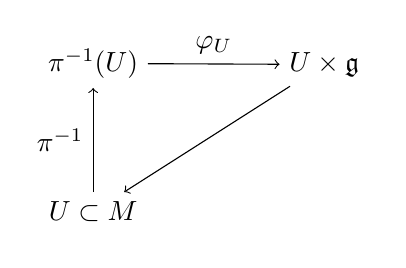
\begin{tikzpicture}
  \matrix (m) [matrix of math nodes, row sep=3.8em, column sep=4.8em, minimum width=2.2em]
  {
\pi^{-1}(U) & U\times \mathfrak{g} \\
U \subset M  & \\
};
  \path[->]
  (m-2-1) edge node [left] {$\pi^{-1}$} (m-1-1)
  (m-1-1) edge node [auto] {$\varphi_U$} (m-1-2) 
  (m-1-2) edge node [auto] {$$} (m-2-1)
;
\end{tikzpicture}
\]
Then for covariant derivative $D_{\mu} :P\to P$,
\[
D_{\mu} \lambda = \partial_{\mu} \lambda + A^c_{ \; \; b\mu} \lambda^b e_c
\]
with $A^c_{\; \; b\mu} (e_c \otimes e^b) dx^{\mu} \in \Omega^1(M;\text{End}(\mathfrak{g}))$, a connection 1-form, in which it (a connection) is a $\text{End}(\mathfrak{g})$-valued 1-form.  

Compare this expression with the one from physics:
\[
D_{\mu} \lambda = \partial_{\mu} \lambda + A^c_{ \; \; b\mu} \lambda^b e_c = \partial_{\mu} \lambda^a T_a + (eA^a_{ \; \; \mu} f_{ab}^{ \; \; c} ) \lambda^b T_c
\]
Thus, what I'll need to check myself more thoroughly, what theorists call the connection 1-form on the principal-$G$ bundle, $A$, is related to what physicists call the gauge field, but in its \emph{adjoint representation}; the clue to why this is the adjoint representation is the $f_{ab}^{ \; \; c}$ factors in $eA^a_{ \; \; \mu} f_{ab}^{ \; \; c}$.  Also, it is unclear to me at least, how to scale or deal with the $e$ numerical factors, which is in the theory.  

\subsubsection{Certain Types of Representations (cf. Hughes, Sec. 6)}

\begin{itemize}
  \item \textbf{trivial representation}: $\rho(g) =0$ \, $\forall \, g\in G$ or $\mathfrak{g}$; $T^a =0$.  $\text{dim}V=1$.  \item \textbf{fundamental representation}: $\rho(g) =g$ \, $\forall \, g\in G$ or $\mathfrak{g}$.  Then $\text{dim}V=N$,  for $g\in \text{Mat}(N,N)$ if $G$ is a ``matrix Lie group'' (similar with $\mathfrak{g}$)   
\item \emph{adjoint representation}: Hughes mentions that $f_{ab}^{ \; \; c}$ are the components of the representation.  Recall that $[T_a,T_b] = f_{ab}^{ \; \; c} T_c$, where $f_{ab}^{ \; \; c}$ are the antisymmetric \emph{structure constants}.  Now $T_a, T_b\in \mathfrak{g}$.  $[T_a,T_b]\in \mathfrak{g}$ ($\mathfrak{g}$ is a Lie algebra, equipped with Lie bracket, by definition).  

So $f_{ab}^{ \; \; c} \in \mathbb{K}$, field $\mathbb{K}$ over which $\mathfrak{g}$ is over with ($\mathbb{K} = \mathbb{R}$ or $\mathbb{C}$ usually).  


\end{itemize}




Redi and Sato (2016) \cite{RS1602} gives a good overall review of the current status of axions in a theory context.


\section{Spin Structures, Fermions (fermionic field) }

The clearest, most lucid, explanation of Spin Geometry is, in my opinion, from Salamon (1996) \cite{Sala1996}: I will interpolate between Salamon (1996) and Jost (2011) \cite{JJost2011}, in particular, Jost's Chapter 2 Lie Groups, Section 2.4 Spin Structures.  

Salamon (1996) \cite{Sala1996} uses $C(V)$ to denote the Clifford Algebra generated by $V$; Jost and Wikipedia uses $Cl(V)$; I'm going to use $Cl(V)$ to stand in for $C(V)$.  

\subsection{Clifford Algebra}


\section{Seiberg-Witten}

$\mathcal{A}$



\begin{thebibliography}{9}

\bibitem{CTaubes2011}
Clifford Henry Taubes, \textbf{Differential Geometry: Bundles, Connections, Metrics and Curvature} (Oxford Graduate Texts in Mathematics, Vol. 23) Oxford University Press; 1 edition (December 1, 2011). ISBN-13: 978-0199605873


%\cite{Witten:1988hf}
\bibitem{Witten:1988hf} 
  E.~Witten,
  ``Quantum Field Theory and the Jones Polynomial,''
  Commun.\ Math.\ Phys.\  {\bf 121}, 351 (1989).
  doi:10.1007/BF01217730
  %%CITATION = doi:10.1007/BF01217730;%%
  %2286 citations counted in INSPIRE as of 24 Feb 2016

\bibitem{DJT1982}
  Deser, S., and R. Jackiw and S. Templeton. \emph{Three-Dimensional Massive Gauge Theories}. \textbf{Phys. Rev. Lett.} \textbf{48}:975.  1982.

  S. Deser, R. Jackiw, and S. Templeton.  ``Three-Dimensional Massive Gauge Theory.'' \textbf{Physical Review Letters}. Volume \textbf{48}, Number 15, 975-978.  12 April 1982.  

  
\bibitem{GW2011}
Davide Gaiotto, Edward Witten. \emph{Knot Invariants from Four-Dimensional Gauge Theory}. 2011.   \href{http://arxiv.org/abs/1106.4789}{arXiv:1106.4789 [hep-th]}


\bibitem{Hick2013}
Kevin Peter Hickerson.  \emph{The physics of ultracold neutrons and Fierz interference in beta decay.}  Dissertation (Ph.D.), California Institute of Technology. 2013.  \url{http://resolver.caltech.edu/CaltechTHESIS:11022012-135115177}


\bibitem{Guko2007}
Sergei Gukov.  ``Gauge theory and knot homologies.''  Fortschr. Phys. \textbf{55}, No. 5 – 7, 473 – 490 (2007) / \textbf{DOI} 10.1002/prop.200610385  \url{http://www.maths.ed.ac.uk/~aar/papers/gukov2.pdf}


\bibitem{RS1602}
Michele Redi, Ryosuke Sato. \emph{Composite Accidental Axions}. \href{arXiv:1602.05427 [hep-ph]}{arXiv:1602.05427} [hep-ph].  \url{http://arxiv.org/abs/1602.05427}




\bibitem{Sala1996}
Dietmar Salamon.  ``Spin Geometry and Seiberg–Witten Invariants.''  1996.  \url{https://people.math.ethz.ch/~salamon/PREPRINTS/witsei.pdf}


\end{thebibliography}

\end{document}

